\RequirePackage{fix-cm}
\documentclass[smallextended]{svjour3}       % onecolumn (second format)
\smartqed  % flush right qed marks, e.g. at end of proof
\usepackage{graphicx,multicol,lipsum,caption,authblk} \usepackage{amsmath,booktabs,verbatim,tikz}
\usepackage{geometry,pgf,pgfplots,}
\usepackage{mathptmx}
\usetikzlibrary{shapes.geometric, arrows,positioning,matrix,calc}
\usetikzlibrary{intersections}
\bibliographystyle{unsrtnat}
% in order to solve arranging citations by order of appearance
\usepackage[numbers]{natbib}
\usepackage{notoccite}
\begin{document}


\title{Selection Schemes Study used in Genetic Algorithm for Multimodal Problem in
Sharing Mechanism}
%\titlerunning{Stacking Sequence Optimization}        % if too long for running head
\author{Zhang Huiyao$^1$  \and
	Atsushi Yokoyama $^{1,*}$
}
\authorrunning{Zhang Huiyao} % if too long for running head
\institute{Zhang Huiyao \at
              Room 203,Bulding 3,Kyoto Institue of Technology\\
			  Matsugasaki,Sakyo-ku,Kyoto,606-8585,JAPAN\\
              \email{zhanghy1012@gmail.com}           %  \\
           \and
           S. Author \at
              second address
}
\date{Received: date / Accepted: date}
\maketitle

\begin{abstract}
    In aritifical intelligence algorithm, Sharing mechanism is widely used in
    genetic algorithm to solve multimodal problems, The number of niches and the
    optimal which were found using share mechanism are highly related with the
    selection method. In this paper, Three common used selection method which
    are Tournament selection Roulette wheel, and ranking selection was analysed.
    The paper analyses consider the three common algorithms and their
    performance for mulimodal problems.
\keywords{Genetic Algorithm \and Niche \and ranking selection \and tournament
selection \and Multimodal}
\end{abstract}

\begin{multicols}{2}

\section{Introduction}
Genetic algorithms (GAs) are first introduced in 1975 by
Holland\cite{sampson1976adaptation}, because of its powerful search ability,
which was widely been used to solve many search, optimiation, and classification
problem. Compared with other artificial integllience search algorithm, for example, particle
swarm optimization, ant colony optimization, and simulated annealing
algorithm\cite{zabinsky2010random}, GAs are not easily trapped in local optima,
and obtain the global optimal.  Traditional GAs has been to successfully find
the optimal value in the domain for unimodal problems, however, sometimes, not
only the optimal point but also the secondary important point is needed.
Because of its search rule, traditional GAs are failed to maintain the
information for a multimodal problem.

For the multimodal problems, the niche sharing mechanism is used to in GA to
find optimal value both in local and global.




\subsection{Genetic Algorithm Procedure}
According to Darwin natural evolution theory, the one who fits the environment
most well are more possilbe to survive and reproduction. GA simulates the
process of natural evolution which includes selection,crossover and mutation.
Because of the powerful search ability of GA,it has been widely used in many
fields for multimodal problems. The procedure diagram of GA as shown in figure
\ref{plot:GA} 
 
\subsection{Parent Selection}
Selection is the most important step of GA algorithm which decides the diversity
of the population. In the step, if the selection pressure increase, the converge
speed of the population increase, however, the diversity of the dopulation
decrease. To improve the search ability and reduce the search cost,
many selection methods \cite{goldberg1991comparative} has been invented,the
selection schemes can be divided into four classes which are proportionate
reproduction, ranking selection, tournament selection and Genitor(or "steady
state") selection.In this paper, to maintain a stable subpopulation for
multimodel problems,the stochastic remainer algorithm is used for experiment,
stochastic remainder algorithm is one of proportional selection method according
to corresponding fitness.

\subsection{Tournament Selection}
Tournament Selection is first comed up by. In a k-way tournament selection,
each member in the tournament are random choosen from parents, and the K string
form the group. Select the best string from the tournament according to their
fitness. The benefifiecnt of this scheme, it increases the diversity of
population. 
\subsection{Roulette Selection}
According to the fitness of each string, assign corresponding probability to the
individual. Then according to the probability of each string, schochastic choose
individual, and pass them to the next generation.
\subsection{Ranking Selection}
Ranking Selection is the method of choosing the parents of next generation from
high to low according to their fitness. The string with best fitness are choosen
as parents, repeat the process until you get the desired amount of
population.the benificiency of this scheme is it keep the individual 


\subsection{Parents Crossover}
According to the selected parents, crossover is used to generate the offspring,
combining genes from parents to reproduce new members. There are so many
research \cite{ahmed2010genetic,nebro2009mocell} about the crossover operation
in GAs to maximize the divistiy of the population. In this paper, one-point
crossover strategy is implemented.

\subsection{Offspring Mutation}
Mutation simulates the situation  genes on the chromosomes which received from
parents randomly changed.  The process are used to provide new evolution
direction and information for the population, the parameters has during this
process has been well researched by Schaffer\cite{schaffer1989study}.  


\subsection{Niched Mechanism}
Niched mechanism simulates another natural process of subpopulation in the
evolutionary process, and introduce the concept niches which means sharing
resource.  Because GA select the best individual according to their fitness, so
the GA converges quickly to find the global optimal value. Howerver, In order to
deal with the multimodal problem, It is significant to maintain the diversity of
the population.  Niched mechanism simulates the There are several methods to
achieve this target,which are Crowding, Deterministic Crowding and Sharing
methods.  share Function\cite{goldberg1987genetic}. In this paper, the
parameters of share function is studied. 
\begin{center}
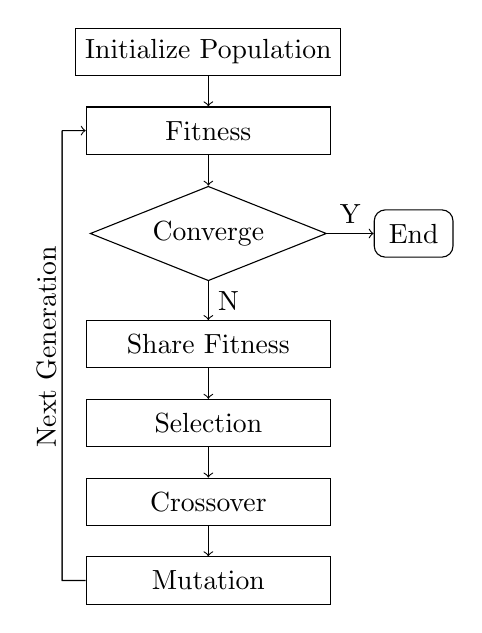
\begin{tikzpicture}
\tikzstyle{startstop} = [rectangle, rounded corners, minimum width=1.0cm,minimum height=0.6cm, 
                        text centered, draw=black]
\tikzstyle{io} = [trapezium, trapezium left angle=70, trapezium right angle=110, minimum width=2cm, 
                 minimum height=0.6cm, text centered, draw=black]
\tikzstyle{process} = [rectangle, minimum width=3.1cm, minimum height=0.6cm, text centered, draw=black]
\tikzstyle{decision} = [diamond,minimum width=3cm, minimum height=1.2cm, draw=black]
\node (population) [process] {Initialize Population};
\node (fitness) [process, below of=population] {Fitness};
\node (decision) [decision] at ($(fitness.south)+(0,-1.0cm)$) {} node at (decision.base) {Converge};
\node (share-fitness) at ($(decision.south)+(0,-0.8cm)$) [process] {Share Fitness};
\node (selection) [process,below of=share-fitness] {Selection};
\node (crossover) [process,below of=selection]  {Crossover};
\node (mutation) [process,below of=crossover]   {Mutation};
\node (end) [startstop] at ($(decision.east)+(1.1cm,0)$)  {End};
\draw [->] (population) -- (fitness);
\draw [->] (fitness) -- (decision);
\draw [->] (decision) -- (share-fitness) node[auto=left,pos=0.5]{N};
\draw [->] (share-fitness.south) -- (selection.north) ;
\draw [->] (selection.south) -- (crossover.north);
\draw [->] (crossover.south) -- (mutation.north);
\draw [->] (decision.east) -- (end.west) node[auto=left,pos=0.5]{Y};

% draw intersection
\draw [white] (fitness.west) -- ++(-0.5cm,0) coordinate (A);
\draw [white] (mutation.west) -- ++(-0.3cm,0) coordinate (B)-- ++(0,6cm) coordinate (C) ; 
\draw (mutation.west) -- ++(-0.3cm,0) -- (intersection cs: first line={(fitness.west)--(A)}, 
      second line={(B)--(C)}) coordinate (D);
\draw (B) -- (D) node[auto=left,pos=0.8,rotate=90,xshift=-0.2cm,yshift=0.2cm] {Next Generation} ;
\draw [<-] (fitness.west) -- (D);
\end{tikzpicture}
\captionof{figure}{GA Procedure with Share Function}
\label{plot:GA}
\end{center}

\subsection{Sharing}
Sharing mechanism is first introduced by Holland \cite{miller1996genetic} to
reduce the fitness of similar individual in the population and increase the
diversity of the population. For Sharing mechanism, the most important thing is
how to identify the number of niches, Miller comed up dynamic niche sharing
method, and lin developed the method to identify the number of niches in the
population.\cite{lin2002niche} The problem within sharing mechanism is how to
identiy the range of parameters in the formula. Given the number of peaks in
population,Deb and Goldberg comed up method to set up the appropriate value for




\section{Research Method}
With the increase of the of size of the population, the GAs are more eazily too
find all the possible possible modal values. so the computation cost will also
increase. In this paper, we focus on with the limited population, to evaluate
the performance of GA, The following three criteria is comed up: 
\subsection{Criteria}
The first evaluation criterion is apparent reliability denoted as $R$, which is
calulate by the following formula
\begin{equation}
R = \frac{n}{\text{N}}
\end{equation}
$n$ stands for the number of GA finds at least one optimal point, $N$ stands for
the number of the runtime of GA. \newline
The second criterion is population richness, denoted as $P_{r}$, which is
calculated by the following formula:
$$
P_{r} = N/P
$$
Population richness is used to denote how many optimal points these GA
maintains. \newline 
The last criterion is the number of niche, denoted by $N_{n}$, the
number of niche can be used to represents the ability of the GA to maintain
subpopluation. \newline
\subsection{Share Function}
Share function is used to increase the diversity of the subpopluation, the
function is shown as Fig.\ref{fig:share}
\begin{equation}
s h\left(d_{i, j}\right)=\left\{\begin{array}{ll}{1-\left(\frac{d_{i, j}}{\sigma_{s h}}\right)^{\alpha_{s h}}} 
    & {\text { if } d_{i, j}<\sigma_{s h}} \\ 
{0} & {\text { otherwise }}\end{array}\right.
\end{equation}
where $d_{i, j}$ denotes distance between two strings, $\alpha_{sh}$ is a contant number,
$\sigma_{sh}$ is also a constant number.

\begin{center}
  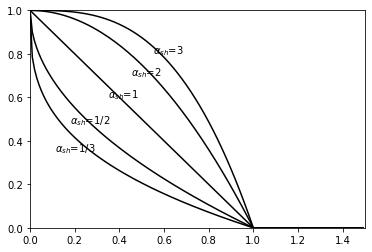
\includegraphics[width=\linewidth]{GA_images/share-function.png}
  \captionof{figure}{Share Function}
  \label{fig:share}
\end{center}



\subsection{GA Parameters}

In order to evaluate the impact of the parameters, the mutation process is
ignored. The parameters of GA is shown in the table \ref{tab:GA}

\begin{center}
\captionof{table}{GA-parameters}
\begin{tabular}{cc}
	\toprule
	parameter & value \\
	\midrule
    runtimes             & 100 \\
	generation           & 50 \\
    encoding length      & 16 \\
    encoding method      & binary encoding\\
	selection strategy   & roulette wheel  \\
	crossover strategy   & one-point \\
	mutation strategy    & None \\
	\bottomrule
\end{tabular}
\label{tab:GA}
\end{center}



The ith individual in the population converted  from binary to decimal by the
following formula:

\begin{equation}
x_i=\frac{\sum_{j=1}^{16}2^{j-1}g_i^j}{2^{15}}
\end{equation}




\section{Experiment and Results}
\subsection{Case 1: Equal stationary value}
In the first experiment, the target function is as shown in the
Eq.\ref{equ:example-1} and the graph is as shown in Fig.\ref{fig:example-1} 
\begin{equation}
f_{1}(x)=\sin^{6}(5.1 \pi x+.5)
\label{equ:example-1}
\end{equation} \newline
As we can see in the in the Fig.\ref{fig:example-1}, There are five niches in
the domain, and all peaks are equal to 1. 
\begin{center}
  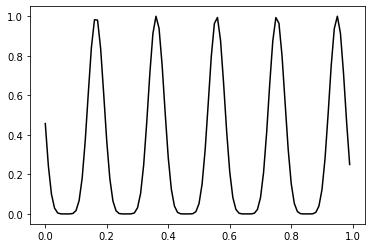
\includegraphics[width=\linewidth]{GA_images/example-sin.png}
  \captionof{figure}{Target Function}
  \label{fig:example-1}
\end{center} 
Tournament selection, roulette selection and ranking selection is taken in the
GA.
The experiment results is shown in the table 
Tab.\ref{tab:tournament-1}
Tab.\ref{tab:roulette-1}
Tab.\ref{tab:ranking-1}

\begin{center}
    \captionof{table}{Tournament Selection}
\begin{tabular}{cccc}
	\toprule
    Population Size      & $R$   &  $P_{r}$ & $N_{n}$\\
	\midrule
    30                   & 0.5  &  0.38   & 2.46 \\
    50                   & 0.78  &  0.87   & 3.17 \\
    70                   & 0.90  &  1.72   & 4.16 \\
    90                   & 0.99  &  2.18   & 4.61 \\
	\bottomrule
\end{tabular}
\label{tab:tournament-1}
\end{center}

\begin{center}
    \captionof{table}{Roulette Selection}
\begin{tabular}{cccc}
	\toprule
    Population Size& $R$   &  $P_{r}$ & $N_{n}$\\
	\midrule
    30& 0.81  &  1.36   & 4.16 \\
    50& 0.95  &  2.11   & 4.55 \\
    70& 1.00  &  2.85   & 4.64 \\
    90& 1.00  &  3.48   & 4.87 \\
	\bottomrule
\end{tabular}
\label{tab:roulette-1}
\end{center}

\begin{center}
    \captionof{table}{Ranking Selection}
\begin{tabular}{cccc}
	\toprule
    Population Size& $R$   &  $P_{r}$ & $N_{n}$\\
	\midrule
    30& 0.82  &  1.41   & 4.31 \\
    50& 0.98  &  2.27   & 4.52 \\
    70& 0.99  &  2.67   & 4.75 \\
    90& 0.99  &  2.79   & 4.84 \\
	\bottomrule
\end{tabular}
\label{tab:ranking-1}
\end{center}

\begin{center}
  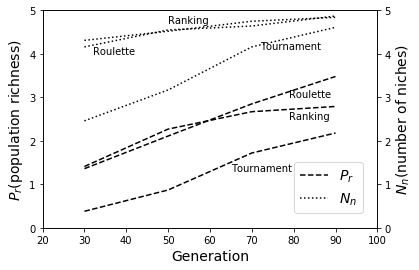
\includegraphics[width=\linewidth]{GA_images/example-case1.png}
  \captionof{figure}{Result 1}
  \label{fig:case1result}
\end{center}

According to the three table, with the increases of the population size, the
population richness $P_r$, The number of best output $O_n$ and the number of
niches $N_n$ decrease,and when $r=1$ and $q=0$,apparent reliability R obtain the
maximaize value,GA obtains the best result.  as shown in Fig.
\ref{fig:sin-result} 

\begin{center}
  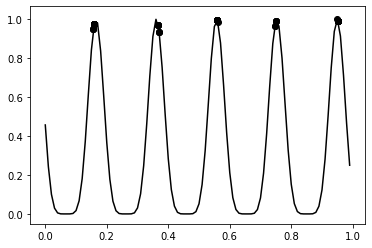
\includegraphics[width=\linewidth]{GA_images/example-sin-result.png}
  \captionof{figure}{Result 1}
  \label{fig:sin-result}
\end{center}


\subsection{Case 2: Non-equal Stationary Value}
In the last experiment, all the function value of the stationary points are
equal. So in this experient the performance of selected scheme is studied for
multimodal problems. The target function is as shown in Eq.\ref{equ-target-2}




\begin{equation}
\mathrm{f}_{2}(\mathrm{x})=\mathrm{f}_{1}(\mathrm{x}) \cdot \mathrm{e}^{\left[-4 \ln 2 \frac{(\mathrm{x}-0.086)^{2}}{0.8^{2}}\right]}
\label{equ-target-2}
\end{equation}

\begin{center}
  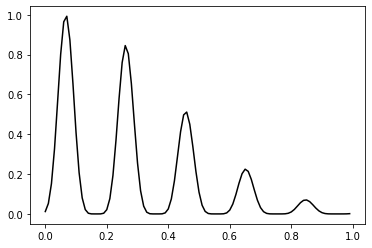
\includegraphics[width=\linewidth]{GA_images/example-composite-sin.png}
  \captionof{figure}{Target}
\end{center}

\begin{center}
    \captionof{table}{Tournament Selection}
\begin{tabular}{cccc}
	\toprule
    Population Size& $R$   &  $P_{r}$ & $N_{n}$\\
	\midrule
    30& 0.69  &  0.52   & 1.74 \\
    50& 0.91  &  1.05   & 2.44 \\
    70& 0.99  &  1.44   & 2.69 \\
    90& 0.98  &  2.45   & 2.84 \\
	\bottomrule
\end{tabular}
\label{tab:case2-generation-30}
\end{center}

\begin{center}
    \captionof{table}{Roulette Selection}
\begin{tabular}{cccc}
	\toprule
    Population Size& $R$   &  $P_{r}$ & $N_{n}$\\
	\midrule
    30& 0.75  &  0.56   & 2.47 \\
    50& 0.94  &  2.11   & 3.07 \\
    70& 1.00  &  2.16   & 3.65 \\
    90& 0.98  &  3.34   & 3.85 \\
	\bottomrule
\end{tabular}
\label{tab:case2-generation-50}
\end{center}

\begin{center}
    \captionof{table}{Ranking Selection}
\begin{tabular}{cccc}
	\toprule
    Population Size& $R$   &  $P_{r}$ & $N_{n}$\\
	\midrule
    30& 0.91  &  1.44   & 2.95 \\
    50& 0.99  &  2.12   & 3.08 \\
    70& 1.00  &  3.24   & 3.34 \\
    90& 1.00  &  4.32   & 3.36 \\
	\bottomrule
\end{tabular}
\label{tab:case2-generation-70}
\end{center}

\begin{center}
  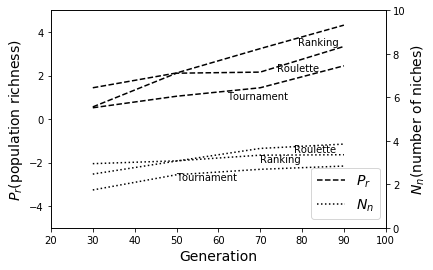
\includegraphics[width=\linewidth]{GA_images/example-case2.png}
  \captionof{figure}{Result 1}
  \label{fig:case2result}
\end{center}

\begin{center}
  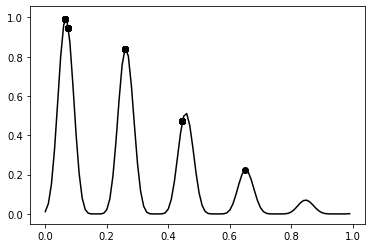
\includegraphics[width=\linewidth]{GA_images/example-composite-sin-result.png}
  \captionof{figure}{Result 2}
\end{center}


\section{Conclusion}
In this paper, the influence of three common selection schemes on sharing
function for two different situations were researched.  The experiment result is measured by three
indexes,apparent reliability population richness, the number of niche
number.According to the experiment, Compared with Ranking selection and Roulette
Selection, the performance of tournament selection are the worst. 
. 

\section{Acknowledgements}
This is work was supported by China Schloarship Council(CSC).

%\bibliographystyle{plain}
\bibliography{ga-citation-database}

\end{multicols}
\end{document}
